\documentclass{beamer}

\mode<presentation>
{
  \usetheme{CambridgeUS}
  \usecolortheme{seagull}
  \setbeamercovered{transparent}
}

\usepackage[english]{babel}
\usepackage[latin1]{inputenc}
\usepackage{times}
\usepackage[T1]{fontenc} 
% Or whatever. Note that the encoding and the font should match. If T1
% does not look nice, try deleting the line with the fontenc.
\usepackage{amsmath}

\newcommand{\linespace}{\vskip 0.25cm}

\definecolor{MyForestGreen}{rgb}{0,0.7,0} 
\newcommand{\tableemph}[1]{{#1}}
\newcommand{\tablewin}[1]{\tableemph{#1}}
\newcommand{\tablemid}[1]{\tableemph{#1}}
\newcommand{\tablelose}[1]{\tableemph{#1}}

\definecolor{MyLightGray}{rgb}{0.6,0.6,0.6}
\newcommand{\tabletie}[1]{\color{MyLightGray} {#1}}

% The text in square brackets is the short version of your title and will be used in the
% header/footer depending on your theme.
\title[Concurrent Compaction in JVM GC]{Concurrent Compaction in JVM Garbage Collection}

% Sub-titles are optional - uncomment and edit the next line if you want one.
% \subtitle{Why does sub-tree crossover work?} 

% The text in square brackets is the short version of your name(s) and will be used in the
% header/footer depending on your theme.
\author[Jacob Opdahl]{Jacob P. Opdahl}


% The text in square brackets is the short version of your institution and will be used in the
% header/footer depending on your theme.
\institute[UMM]
{
  University of Minnesota, Morris \\[\baselineskip]
  \emph{opdah023@morris.umn.edu}
}

% The text in square brackets is the short version of the date if you need that.
\date[December 5, 2015] % (optional)
{December 5, 2015}

% Delete this, if you do not want the table of contents to pop up at
% the beginning of each subsection:
%\AtBeginSection[]
%{
%  \begin{frame}<beamer>
%    \frametitle{Outline}
%    \tableofcontents[currentsection, hideothersubsections]
%  \end{frame}
%}

\begin{document}

\begin{frame}
  \titlepage
\end{frame}

% For a 20-25 minute senior seminar talk you probably want something like:
% - Two or three major sections (other than the summary).
% - At *most* three subsections per section.
% - Talk about 30s to 2min per frame. So there should probably be between
%   15 and 30 frames, all told.



\section*{Overview}

\subsection*{Garbage Collection}

%\begin{frame}
%\end{frame}



\subsection*{Outline}

\begin{frame}
  \frametitle{Outline}
  \tableofcontents  
  %\tableofcontents[hidesubsections]
\end{frame}



\section[Introduction]{Introduction}

\subsection[GC Basics]{Garbage Collection Basics}

%Kristin liked the heap visualization I did when explaining it (did with my hands at the time).

\subsection[PP Basics]{Parallel Processing Basics}



\subsection[GC with PP]{Garbage Collection with Parallel Processing}



\section[C4]{Continuously Concurrent Compacting Collector (C4)}

\subsection*{Explanation}



\subsection*{Test Results}



\section[Collie]{Collie Collector}

\begin{frame}

\frametitle{The Collie Garbage Collector}

Collie is a full garbage collector
\begin{itemize}
\item Uses most techniques from C4
\end{itemize}

\linespace

Also intended for server environments

\linespace

Uses transactional memory for synchronization

\linespace

Major focus on improving latency

\linespace
\linespace
\linespace

\begin{center}
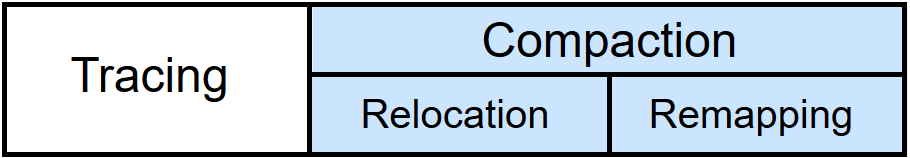
\includegraphics[width=.85\textwidth]{Illustrations/gc_cycle_locator_compaction.png}
\end{center}

\end{frame}



\subsection*{Explanation}

\begin{frame}

\frametitle{Transactions}

%Remember to emphasize the key point is interruptions will cause nothing to happen, or everything to.
\emph{transaction}: series of operations performed in an all-or-none manner

\linespace
\linespace

Example: updating prices in a store for sales \\
\begin{itemize}
\item Update sale price
\item Update store price
\end{itemize}

\linespace

Protects data from interrupts

\linespace
\linespace

\emph{transactional memory}: allows code sections to run like transactions
\begin{itemize}
\item Memory used by the code is protected
\end{itemize}

\end{frame}

\begin{frame}

\frametitle{Transplantations}

\emph{transplantation}: Relocating and remapping unmodified objects

\linespace
\linespace

\begin{columns}
\begin{column}{0.33\textwidth}

Transaction:
\begin{itemize}
\item Start transaction
\item Check object
\item Relocate object
\item Remap references
\item End Transaction
\end{itemize}

\end{column}
\begin{column}{0.32\textwidth}


$\xrightarrow{\text{Interrupted by application}}$

\end{column}
\begin{column}{0.3\textwidth}

Mark object as non-individually transplantable

\end{column}
\end{columns}

\end{frame}

\begin{frame}

\frametitle{Leftovers}



\end{frame}



\subsection*{Test Results}

\begin{frame}

\frametitle{Testing Environment}



\end{frame}

\begin{frame}

\frametitle{Results}



\end{frame}



\section[FPP]{Field Pinning Protocol}

\begin{frame}

\frametitle{Field Pinning Protocol}

Solely describes concurrent relocation

\linespace
\linespace

Implements into a host garbage collector
\begin{itemize}
\item Designed for flexibility
\end{itemize}

\linespace
\linespace

Performs relocation without barriers!

\linespace
\linespace
\linespace
\linespace

\begin{center}
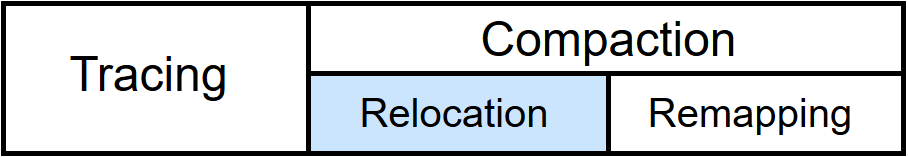
\includegraphics[width=.85\textwidth]{Illustrations/gc_cycle_locator_relocation.png}
\end{center}

\end{frame}



\subsection*{Explanation}

\begin{frame}

\frametitle{Hazard Pointers}

Point to objects an application thread is accessing
\begin{itemize}
\item \emph{Pin} the object
\end{itemize}

\linespace
\linespace

Inform other threads of objects that are in use

\linespace
\linespace

Are maintained by the thread they belong to

\linespace
\linespace

Main goal: safely access objects without worrying about relocation

%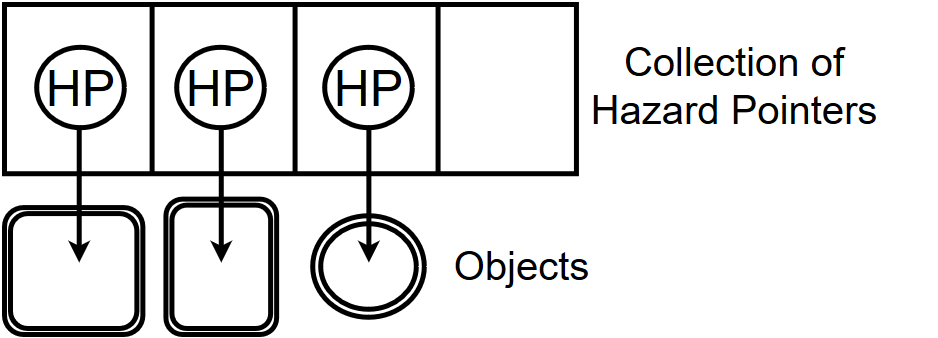
\includegraphics[width=.95\textwidth]{Illustrations/FPP_HP_Illustration.png}


\end{frame}


\begin{frame}

\frametitle{Example}

\begin{columns}
\begin{column}{0.45\textwidth}
	\begin{itemize}
	\item Object = Coffee 
	\item \color{red}{Application Thread = Person w/ Coffee Cup} 
	\only<2->{\item \color{blue}{Relocation Thread = Person}}
	\only<2->{\item \color{black}{* = Responsible}} 
	\only<2->{\item ! = Impeded}
	\end{itemize}
\end{column}
\begin{column}{0.55\textwidth}
	\only<1>{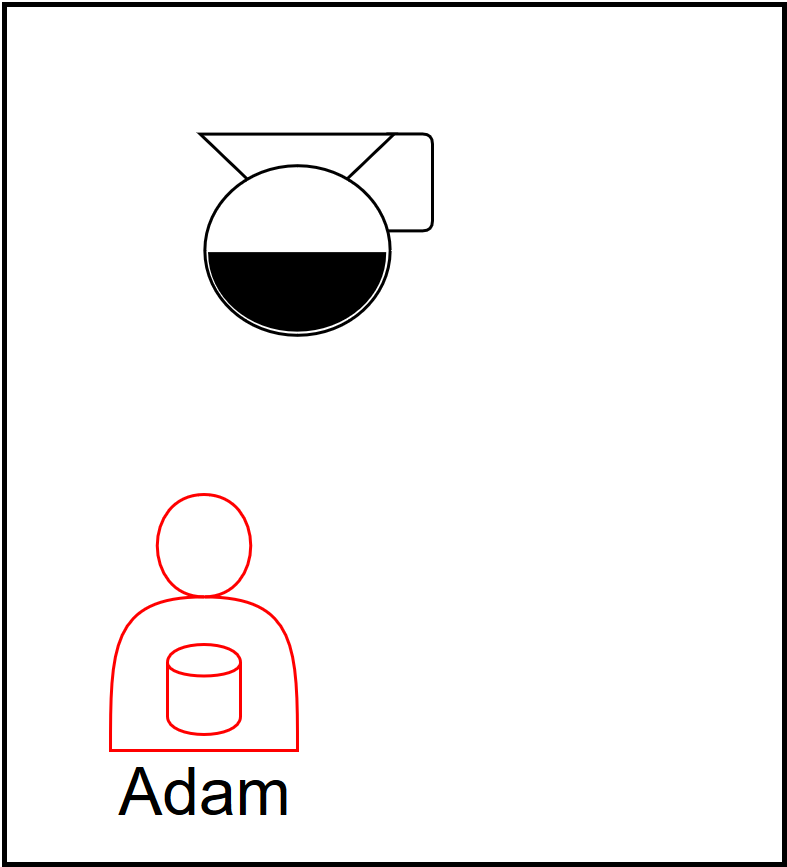
\includegraphics[width=.95\textwidth]{Illustrations/coffeeLineNew1.png}}
	\only<2>{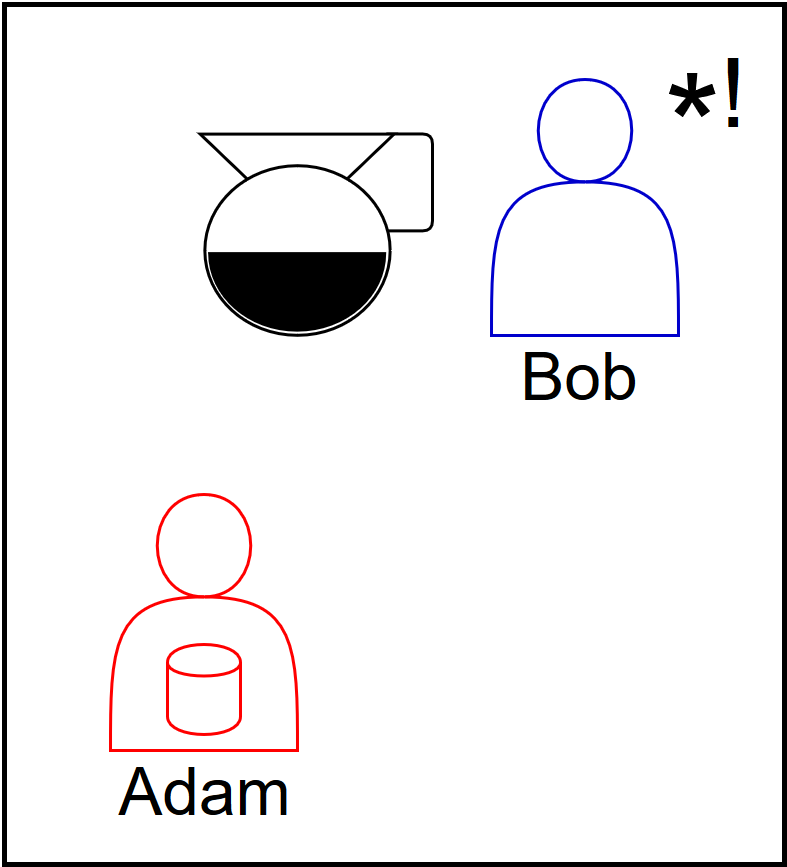
\includegraphics[width=.95\textwidth]{Illustrations/coffeeLineNew2.png}}
	\only<3>{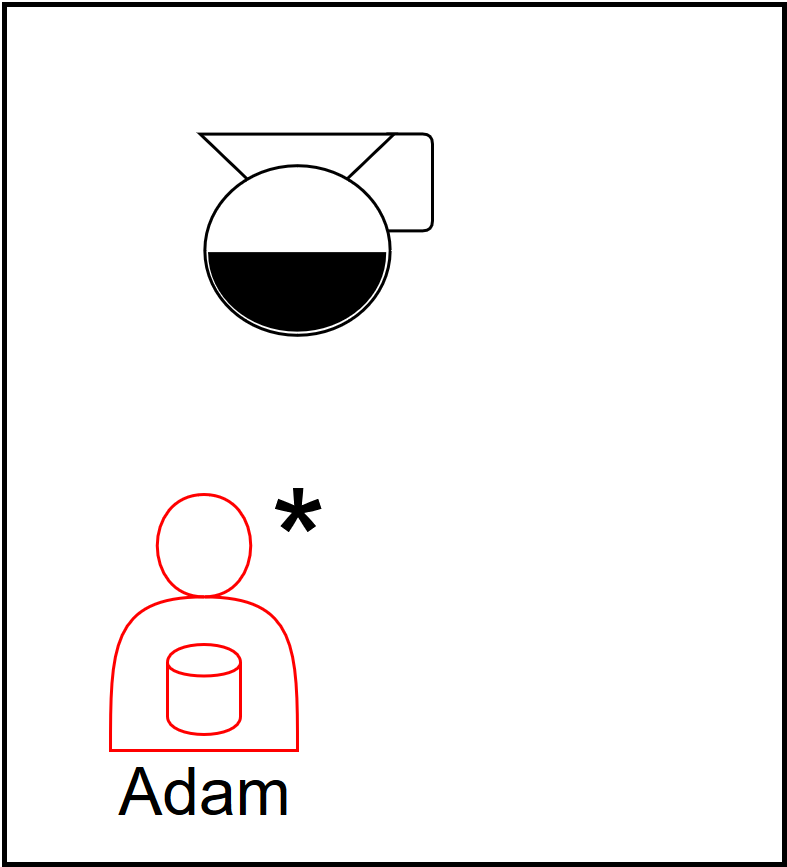
\includegraphics[width=.95\textwidth]{Illustrations/coffeeLineNew3.png}}
	\only<4>{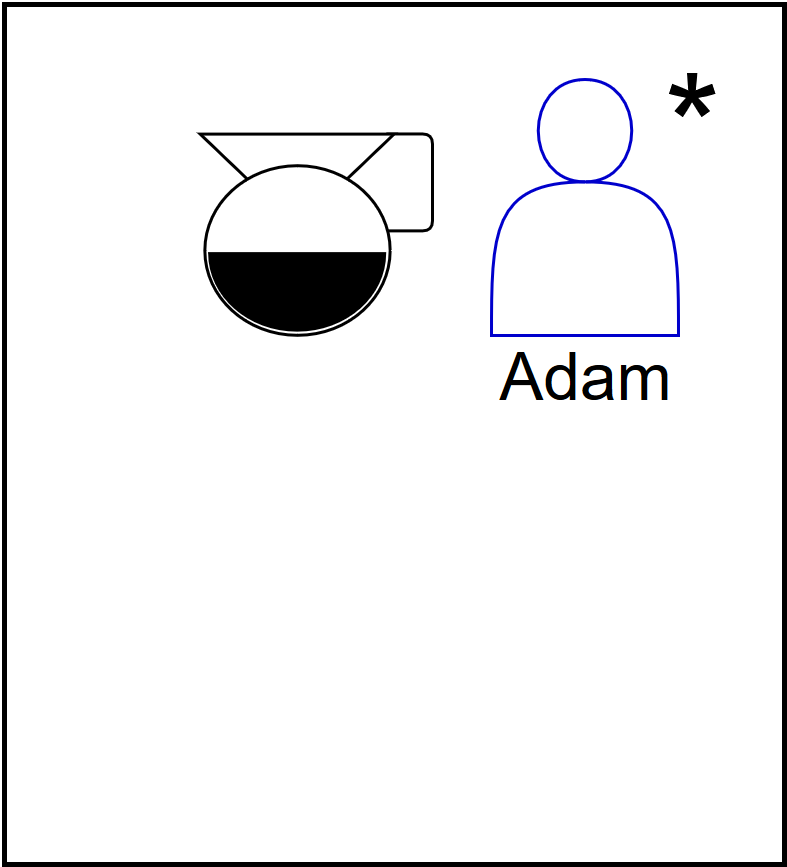
\includegraphics[width=.95\textwidth]{Illustrations/coffeeLineNew4.png}}
	\only<5>{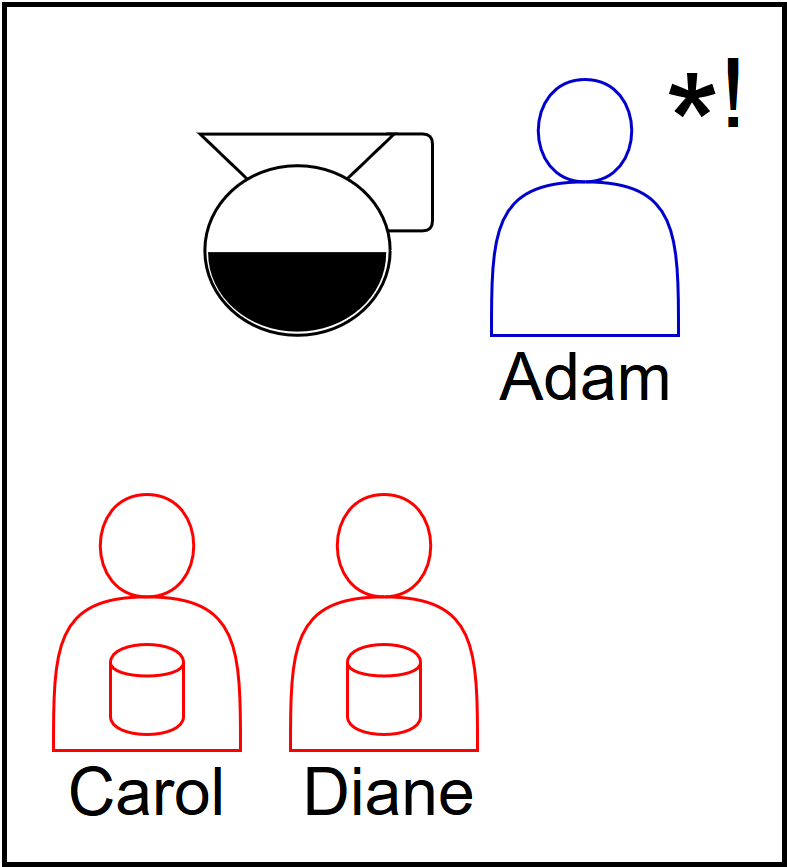
\includegraphics[width=.95\textwidth]{Illustrations/coffeeLineNew5.png}}
\end{column}
\end{columns}

\end{frame}


\begin{frame}

\frametitle{The Blame Game}

%If time allows and feedback demands, could break this into multiple slides to not have so much text
%on one as well as to refer back to the example and characters more.

\emph{blamed} thread: responsible for relocating an object
\begin{itemize}
\item Comes from hazard pointers (coffee cups) impeding copying
\end{itemize}

\linespace
\linespace

When relocation begins:
\begin{itemize}
\item GC threads attempt to relocate objects
\begin{itemize}
\item No blame passed!
\end{itemize}
\item GC threads try again
\begin{itemize}
\item Blame interrupting threads
\end{itemize}
\item Blame passed to interrupting threads until relocation succeeds
\end{itemize}

\end{frame}


\begin{frame}

\frametitle{An Application Thread's Perspective}

Process followed by an \color{red}{application thread}\color{black}{:}
\linespace

\begin{columns}
\begin{column}{0.5\textwidth}
\begin{enumerate}
\item Pin object with a hazard pointer
\item Check if the object has been moved already
\item Use the object without worry
\item Unpin the object when done
\item If blamed, try to relocate the object
\end{enumerate}
\end{column}

\begin{column}{0.5\textwidth}
\begin{enumerate}
\item Get a coffee cup
\item Check that the coffee is still in the room
\item Drink all the coffee you want
\item Discard your coffee cup
\item If blamed, try to move the coffee
\end{enumerate}
\end{column}
\end{columns}

\end{frame}



\subsection*{Test Results}

\begin{frame}

\frametitle{Testing Environment}

Implemented in the Garbage-First (G1) Garbage Collector
\begin{itemize}
\item Concurrent tracing
\item Compaction requires stop-the-world pauses
\end{itemize}

\linespace

Tested against the default G1 collector

\linespace

Standard JVM benchmarks used to test latency
\begin{itemize}
\item Concurrent relocation improvements to latency seen
\end{itemize}

%\todo[inline]{Add image here just showing where FPP gets inserted into the overall GC cycle.}

\end{frame}

\begin{frame}

\frametitle{Results}

%Show the figures from the paper here and start talking about them
\only<1>{
\begin{center}
Average GC Pauses for Various Benchmarks
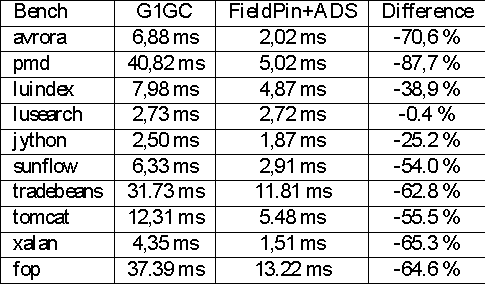
\includegraphics[width=.80\textwidth]{Illustrations/fpp_results.pdf}
\end{center}
}

\only<2>{
\begin{columns}
\begin{column}{0.5\textwidth}

\color{red}G1 with FPP \color{black}on average 50\% shorter pauses than \color{blue}standard G1\color{black}
\begin{itemize}
\item Less impact on application thread performance
\end{itemize}

\linespace

Most latency from host activities

\linespace

Concurrent relocation without barriers is feasible

\end{column}

\begin{column}{0.5\textwidth}
\begin{center}
Average GC Pauses
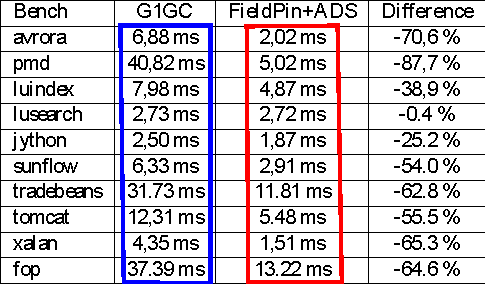
\includegraphics[width=.90\textwidth]{Illustrations/fpp_results_2.pdf}
\end{center}
\end{column}
\end{columns}
}

%In the same slide using 'only', show the images (smaller), with text explaining the results

\end{frame}



\section[Conclusions]{Conclusions}

\begin{frame}
	\frametitle{Thanks for your time!}
	
	\begin{center}
	{\huge Questions?}
	\end{center}	
	
	\linespace
	\linespace	
	
	\begin{center}
	Contact: opdah023@morris.umn.edu
	\end{center}
	
\end{frame}



\section*{References}

\begin{frame} 
	\frametitle{References} 
	
%	\begin{thebibliography}{lskdjf}
%	
%	\bibitem{McPhee:2009:gecco}
%N.~F. McPhee, E.~Crane, S.~Lahr, and R.~Poli.
%\newblock Developmental Plasticity in Linear Genetic Programming.
%\newblock In G\"unther Raidl, \emph{et al}, editors, {\em GECCO '09}, pages 1019--1026, Montr\'eal, Qu\'ebec, Canada, 2009.
%	
%	\bibitem{citeulike:3452411}
%	R.~Poli and N.~McPhee.
%\newblock A linear estimation-of-distribution {GP} system.
%\newblock In M.~O'Neill, \emph{et al}, editors, {\em EuroGP 2008}, volume
%  4971 of {\em LNCS}, pages 206--217, Naples,
%  26-28 Mar. 2008. Springer.
%  
%  	\end{thebibliography}
%	
%	\linespace
%	\begin{center}
%	See the GECCO '09 paper for additional references.
%	\end{center}

\begin{thebibliography}{lskdjf}

\bibitem{Lowe:2015}
E.~\"{O}sterlund and W.~L\"{o}we.
\newblock Concurrent compaction using a field pinning protocol. 
\newblock 2015 ACM SIGPLAN International Symposium on Memory Management (ISMM 2015). ACM, New York, NY, USA, 56-69.

\end{thebibliography}

\end{frame} 



\end{document}


